\begin{activity} \label{A:1.6.2}
This activity builds on our experience and understanding of how to sketch the graph of $f'$ given the graph of $f$.  

\begin{figure}[h]
\begin{center}
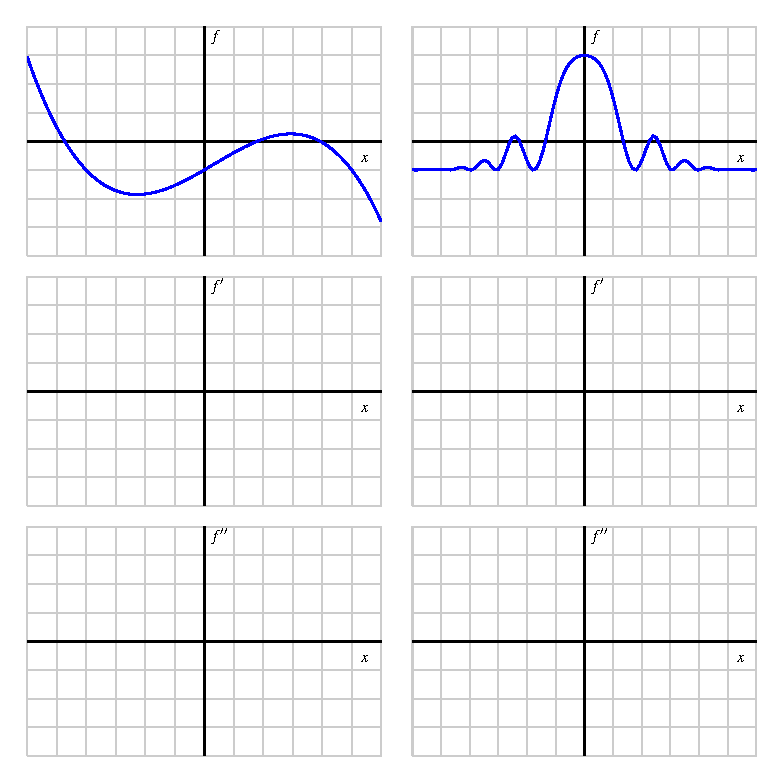
\includegraphics{figures/1_6_Act2.eps}
\caption{Two given functions $f$, with axes provided for plotting $f'$ and $f''$ below.} \label{F:1.6.A2}
\end{center}
\end{figure}

\noindent In Figure~\ref{F:1.6.A2}, given the respective graphs of two different functions $f$, sketch the corresponding graph of $f'$ on the first axes below, and then sketch $f''$ on the second set of axes.  In addition, for each, write several careful sentences in the spirit of those in Activity~\ref{A:1.6.1} that connect the behaviors of $f$, $f'$, and $f''$.  For instance, write something such as
\begin{quote}
$f'$ is \underline{\hspace{1.5in}} on the interval \underline{\hspace{0.5in}}, which is connected to the fact that $f$ is \underline{\hspace{1.5in}} on the same interval \underline{\hspace{0.5in}}, and $f''$ is \underline{\hspace{1.5in}} on the interval as well
\end{quote}
but of course with the blanks filled in.  Throughout, view the scale of the grid for the graph of $f$ as being $1 \times 1$, and assume the horizontal scale of the grid for the graph of $f'$ is identical to that for $f$.  If you need to adjust the vertical scale on the axes for the graph of $f'$ or $f''$, you should label that accordingly.

\end{activity}
\begin{smallhint}
Remember that to plot $y = f'(x)$, it is helpful to first identify where $f'(x) = 0.$
\end{smallhint}
\begin{bighint}
Remember that to plot $y = f'(x)$, it is helpful to first identify where $f'(x) = 0$, and then ask where $y = f'(x)$ is positive and negative.  In a similar way, once $y = f'(x)$ has been plotted, to construct the graph of $y=f''(x)$, it is useful to note where the slope of the tangent line to $y = f'(x)$ is zero, as well as where such slopes are positive and negative.  Heights on the graph of $y = f''(x)$ will correspond to slopes on $y = f'(x)$.
\end{bighint}
\begin{activitySolution}
The graphs of $f'$ and $f''$ are plotted in Figure~***.
%%%%HMMM
%\begin{figure}[h]
%\begin{center}
%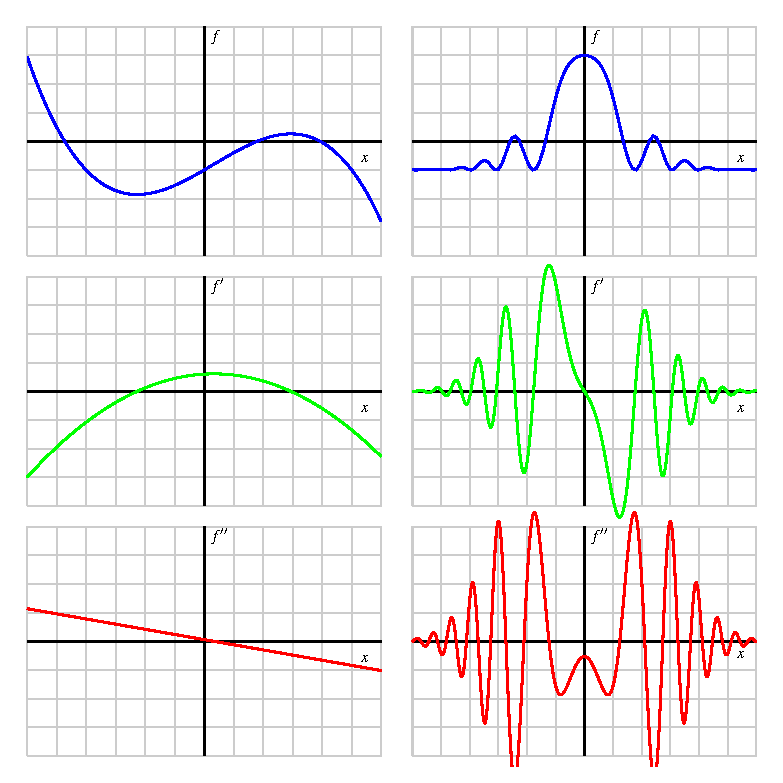
\includegraphics{figures/1_6_Act2Soln.eps}
%\caption{Two given functions $f$, with axes provided for plotting $f'$ and $f''$ below.} \label{F:1.6.A2Soln}
%\end{center}
%\end{figure}
%plus commentary after updating the figure
\end{activitySolution}
\aftera